\documentclass[../../HW02.tex]{subfiles}

\begin{document}
\begin{center}
    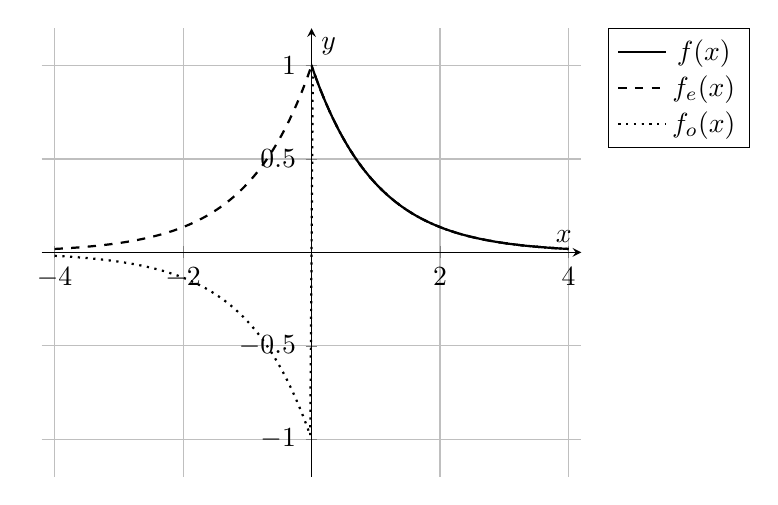
\begin{tikzpicture}
        \begin{axis}[
                axis lines=middle,
                grid=both,
                xmin=-4.2, xmax=4.2,
                ymin=-1.2, ymax=1.2,
                samples=200,
                xlabel={$x$},
                ylabel={$y$},
                legend style={at={(1.05,1)},anchor=north west}
            ]

            \addplot[thick,domain=0:4] {exp(-x)};
            \addlegendentry{$f(x)$}

            \addplot[thick,domain=-4:4,dashed] {exp(-abs(x))};
            \addlegendentry{$f_e(x)$}

            \addplot[thick,domain=-4:4,dotted]
            { (x==0 ? 0 : (x>0 ? exp(-x) : -exp(x))) };
            \addlegendentry{$f_o(x)$}

        \end{axis}
    \end{tikzpicture}
\end{center}
\begin{align*}
    f_c(x)          & =\int_{0}^{\infty}A(\lambda)\cos(\lambda x)\,d\lambda                                                                                \\
    A(\lambda)      & = \frac{2}{\pi} \int_{0}^{\infty} f(x)\cos(\lambda x)\,dx                                                                            \\
    A(\lambda)      & = \frac{2}{\pi} \int_{0}^{\infty} e^{-x}\cos(\lambda x)\,dx                                                                          \\
    I               & = \int_{0}^{\infty} e^{-x}\cos(\lambda x)\,dx                                                                                        \\
    I               & = \left. -e^{-x}\cos(\lambda x)  \right|_0^\infty - \int_{0}^{\infty} e^{-x}\lambda \sin(\lambda x)\,dx                              \\
    I               & = 1 - \lambda \int_{0}^{\infty} e^{-x}\sin(\lambda x)\,dx                                                                            \\
    I               & = 1 - \lambda \left[ \left. -e^{-x}\sin(\lambda x)\right|_0^\infty - \int_{0}^{\infty} -e^{-x}\lambda \cos(\lambda x)\,dx \right]    \\
    I               & = 1 + \cancelto{0}{\left. \lambda e^{-x} \sin(\lambda x) \right|_0^\infty } - \lambda^2 \int_{0}^{\infty} e^{-x} \cos(\lambda x)\,dx \\
    I               & = 1 - \lambda^2 I                                                                                                                    \\
    I + \lambda^2 I & = 1                                                                                                                                  \\
    I               & = \frac{1}{1 + \lambda^2}                                                                                                            \\
    f_c(x)          & = \int_{0}^{\infty}\frac{2}{\pi}\left[ \frac{1}{1 + \lambda^2} \right] \cos(\lambda x)\,d\lambda                                     \\
    f_c(x)          & = \boxed{\frac{2}{\pi}\int_{0}^{\infty}\frac{\cos(\lambda x)}{1 + \lambda^2}\,d\lambda}
\end{align*}
\begin{align*}
    f_s(x)          & = \int_{0}^{\infty}B(\lambda)\sin(\lambda x)\,d\lambda                                                                         \\
    B(\lambda)      & = \frac{2}{\pi} \int_{0}^{\infty} f(x)\sin(\lambda x)\,dx                                                                      \\
    B(\lambda)      & = \frac{2}{\pi} \int_{0}^{\infty} e^{-x} \sin(\lambda x)\,dx                                                                   \\
    I               & = \int_{0}^{\infty} e^{-x} \sin(\lambda x)\,dx                                                                                 \\
    I               & = \left. -e^{-x}\sin(\lambda x)\right|_0^\infty - \int_{0}^{\infty} e^{-x} \lambda \cos(\lambda x) \, dx                       \\
    I               & = \cancelto{0}{\left. -e^{-x}\sin(\lambda x)\right|_0^\infty} - \lambda \int_{0}^{\infty} e^{-x} \cos(\lambda x) \, dx         \\
    I               & = \lambda \left[ \left. -e^{-x} \cos(\lambda x) \right|_0^\infty - \int_{0}^{\infty} e^{-x}\lambda \sin(\lambda x)\,dx \right] \\
    I               & = \lambda \left[ -1 - \lambda \int_{0}^{\infty} e^{-x}\sin(\lambda x)\, dx \right]                                             \\
    I               & = -\lambda - \lambda^2 I                                                                                                       \\
    I + \lambda^2 I & = -\lambda                                                                                                                     \\
    I               & = \frac{-\lambda}{1 + \lambda^2}                                                                                               \\
    f_s(x)          & = \int_{0}^{\infty} \frac{2}{\pi} \left[ \frac{-\lambda}{1 + \lambda^2} \right]\sin(\lambda x)\,d\lambda                       \\
    f_s(x)          & = \boxed{\frac{2}{\pi} \int_{0}^{\infty} \frac{-\lambda \sin(\lambda x)}{1 + \lambda^2}\,d\lambda}
\end{align*}
\end{document}